\chapter{Circuit Results Discussion and Summary}
This chapter presents the results of our read-out circuit and the summary of this thesis.

\section{The Fronted Circuit and DC-sweep mode}
\begin{figure}[tbh!]
    \centering
        \includegraphics[width=0.5\textwidth] {images/chapter6/FrontedCircuit.png}
    \caption{The fronted circuit}
    \label{fig:frontedCIrcuit}
\end{figure}
As in Fig.\ref{fig:frontedCIrcuit}(a), the fronted circuit includes a biasing current source (Ibias), transimpedance amplifier (TIA) and an operational amplifier (OP).
These three circuit blocks combined with the nanowire device (SiNW) form a feedback structure, which is DC-sweep mode of our circuit.

\subsection{Ibias}
\begin{figure}[tbh!]
    \centering
        \includegraphics[width=0.25\textwidth] {images/chapter5/mirror.PNG}
    \caption{The Ibias circuit}
    \label{fig:mirror_ch6}
\end{figure}
The Fig.\ref{fig:mirror_ch6} is the schematic of the Ibias circuit.
The relation between the resistance of the external resistor and the biasing current is shown in Fig.\ref{fig:chip:mirror}.
The Ibias circuit is able to provide a biasing current from $100n A$ to $50\mu A$ stably.
It should be noted that this biasing current range binds the operational range of DC-sweep mode circuit.

\begin{figure}[tbh!]
    \centering
        \includegraphics[width=0.6\textwidth]{images/chapter6/Ibias.png}
    \caption{The relation between biasing current ($I_{bias}$) and resistance of the external resistor}
    \label{fig:chip:mirror}
\end{figure}

\subsection{TIA}
The Fig.\ref{fig:chip:TIA}(a) and (c) show that the dynamic input current range of TIA is $+5.3\mu A \sim -15\mu A$.
The Fig.\ref{fig:chip:TIA}(b) and (d) are the respective derivative ($\frac{\partial V_{out}}{\partial I_{in}}$)
As illustrated in these figures, the transimpedance of TIA is $103k$.
It is notable that not all TIA on the chips have the same transimpedance.
This is because the transimpedance value depends on the resistance of the resistor in TIA (Fig.\ref{fig:frontedCIrcuit}).
This resistor is made of N-well, which should have the largest resistance-to-surface ratio among other kinds of resistor.
But since the doping concentration may vary with the fabrication process, such kind of resistor has a larger resistance variance (\% 30).
We have performed necessary simulations before tap out.
It is assured that the variance does not disturb the important properties of whole read-out circuit such as stability and noise ratio.

\begin{figure}[tbh!]
    \centering
    \begin{minipage}[t]{0.8\textwidth}
        \includegraphics[width=1\textwidth]{images/chapter6/Trimp_I+.png}
        \raggedleft
    \end{minipage}
    \hfill
    \centering
    \begin{minipage}[t]{0.8\textwidth}
        \includegraphics[width=1\textwidth]{images/chapter6/Trimp_I-.png}
        \raggedleft
    \end{minipage}
    \caption{The dc simulation results of TIA. The x-axis represents positive/negative input current (log scale). \textbf{(a)} is the $V_{out}$ responding to the positive input current while \textbf{(c)} is to the negative input current.
                    \textbf{(b)} and \textbf{(d)} are the partial derivative of $V_{out}$ with respect to input current ($\frac{\partial V_{out}}{\partial {I_{in}}}$) from (a) and (c) respectively.}
    \label{fig:chip:TIA}
\end{figure}




\subsection{OP} \label{sec:ch6:OP}
A sinusoidal signal is sent to the negative input of OP and the output signal is measured in Fig.\ref{fig:chip:OPGain}.
It shows that the gain of the feedback OP is only about $1k$.
However, the gain of OP was designed to be more than $5k$.
We will discuss this problem in the following section.

\begin{figure}[tbh!p]
    \centering
        \includegraphics[width=0.8\textwidth] {images/chapter6/Problem_OPGain.png}
    \caption{The output voltage of the feedback OP when the negative input is applied with a sinusoidal signal.
            This input sinusoidal signal has frequency of $1$Hz and amplitude of $2m V$.
            The positive input of OP is biased with a constant voltage generated by the chip (VRef in Fig.\ref{fig:chip:DCmode}).
            The output signal has amplitude around $2 V$, which means that the gain of OP is about $1k$.}
    \label{fig:chip:OPGain}
\end{figure}

\subsection{Measurement with DC-sweep Mode Circuit and the Low-current Defect Problem}
\begin{figure}[tbh!]
    \centering
        \includegraphics[width=0.5\textwidth] {images/chapter6/DCMode.png}
    \caption{DC-sweep mode circuit}
    \label{fig:chip:DCmode}
\end{figure}

With DC-sweep mode (Fig.\ref{fig:chip:DCmode}), Ibias is swept and $V_G$ and $I_D$ are measured to obtain the $I_D$-$V_G$ and $I_{bias}$-$V_G$ curves (Fig.\ref{fig:chip:IdIbiasVG}).
The chip works well when $I_{bias}$ is larger than $1\mu A$.
The overlap between two curves implies that $I_D$ follows $I_{bias}$ and $V_G$ consequently alters owing to the feedback mechanism.

When current becomes low, the circuit fails to prompt nanowire to follow the biasing current.
This phenomenon could be reasonable because lower $I_D$ implies lower $g_m$ and the feedback ability of the circuit may be not strong enough to push the gate of nanowire.
However we expected this happens for $g_m$ below $200n$.
The Fig.\ref{fig:chip:gmId} indicates that the this happens when $g_m$ is less than $5\mu$ instead.
We call this problem as low-current defect problem.

\begin{figure}[tbh!]
    \centering
    \includegraphics[width=0.8\textwidth] {images/chapter6/gvt_0101Manual_IdVg.png}
    \caption{The measurement result of DC-sweep mode circuit. $I_{bias}$ is the biasing current. $I_D$ is the current flowing through the nanowire device.
    One can observe a separation between two curves in low current section ($< 1\mu A$).}
    \label{fig:chip:IdIbiasVG}
\end{figure}

\begin{figure}[tbh!]
    \centering
        \includegraphics[width=0.7\textwidth] {images/chapter6/gvt_0101Manual_gmId.png}
    \caption{The $g_m$-$I_D$ curve. It is obtained from the $I_D$-$V_G$ curve in Fig.\ref{fig:chip:IdIbiasVG}.
            ``Circuit fails'' means the two curves in Fig.\ref{fig:chip:IdIbiasVG} are separated where ``circuit works'' means they are overlapped.}
    \label{fig:chip:gmId}
\end{figure}

\subsubsection*{Insufficient Gain}
We first suspected that it is caused by the insufficient gain of the feedback OP.
According to the last section (Section.\ref{sec:ch6:OP}), the gain is about $1k$.
The discussion in Section.\ref{sec:feedM} suggests that the feedback mechanism depends on the loop gain.
The loop gain should be larger than 100 for DC-sweep mode being functional.
Based on Eq.(\ref{eq:TF_RA}) and Eq.(\ref{eq:TF_LG}), if $A_{OP}$ is $1k$, the loop gain drops below 100 when $g_m$ is less than $1\mu$.
In other words, even though the gain of OP is 5 fold smaller than the gain we designed, the circuit should work well when $g_m$ is larger than $1\mu$.
But in fact, the circuit fails for $gm$ below $5\mu$.

One possible reason is that the gain of OP varies with input.
Fig.\ref{fig:chip:line} is the illustration of the input-output response of the feedback OP.
As depicted by it, the slope ($\frac{\partial V_{out}}{V_{input}}$) in the midst of the curve is larger than the slope at the both ends (The slope can represent the gain of OP).
In the measurement of Fig.\ref{fig:chip:OPGain}, the offset of the output signal is around $2V$.
But in Fig.\ref{fig:chip:IdIbiasVG}, when the separation happens, the output voltage of OP ($V_G$) is less than $1.5V$.
Thus, we assert that the gain of OP is less than we measured.

\begin{figure}[tbh!]
\centering
    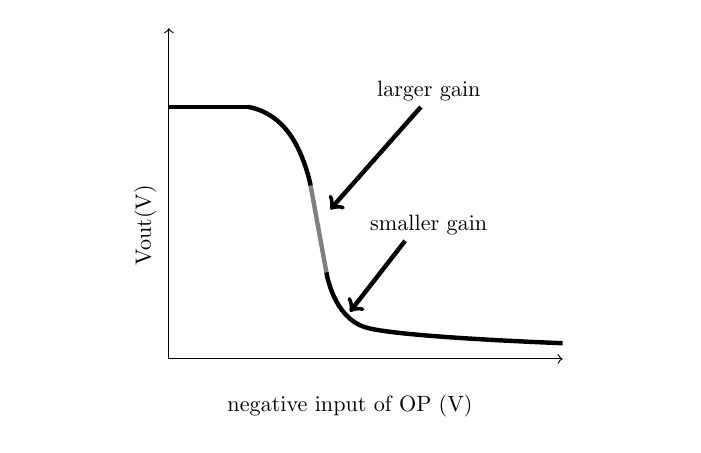
\begin{tikzpicture}
        \draw [black, ultra thick] plot coordinates { (0,4) (1,4) };
        \draw [black, ultra thick] plot [smooth, tension=1] coordinates { (1,4) (1.5,3.7) (1.8,3) };
        \draw [gray, ultra thick] plot [smooth, tension=1] coordinates { (1.8,3) (2,1.9) };
        \draw [black, ultra thick] plot [smooth, tension=0.5] coordinates { (2,1.9) (2.5,1.2) (5, 1) };

        \draw[->] (0, 0.8) -- (0, 5);
        \draw[->] (0, 0.8) -- (5, 0.8);
        \draw[->, ultra thick] (3.2, 4) -- (2.05,2.7);
        \draw[->, ultra thick] (3, 2.3) -- (2.3,1.4);
        \node[text width=5cm, scale=0.8, align=center] at (3.3, 2.5)
            {smaller gain};
        \node[text width=5cm, scale=0.8, align=center] at (3.3, 4.2)
            {larger gain};
        \node[text width=10cm, scale=0.8, align=center] at (2.3, 0.2)
            {negative input of OP (V)};
        \node[text width=5cm, scale=0.8, align=center, rotate=90] at (-0.3, 2.5)
            {Vout(V)};
    \end{tikzpicture}
    \caption{The illustration of the input-output response of the feedback OP.}
    \label{fig:chip:line}
\end{figure}


\subsubsection*{Input Offset Voltage}
Another reason may be responsible for the low-current defect is the offset voltage at the input of the feedback OP.

The output voltage of TIA ($V_{TIA}$) of the DC-sweep experiment in Fig.\ref{fig:chip:IdIbiasVG} is examined and shown in Fig.\ref{fig:chip:VTIA}.
Ideally, when feedback mechanism works well, $V_{TIA}$ should be equal to $V_{Ref}$(Fig.\ref{fig:chip:DCmode}).
However, the value of $V_{Ref}$ is $0.802 V$, which is smaller than $V_{TIA}$.
(This $V_{Ref}$ is connected to a constant voltage point inside the chip.
its value is known indirectly by measuring the drain voltage of nanowire since the drain of nanowire is kept to be same as $V_{Ref}$ by TIA.)
When the circuit works well, $V_{TIA}$ and $V_{Ref}$ is still different by $15m V$.
This voltage difference can result in a $150n A$ offset current flowing through TIA and into the nanowire device.
This offset current becomes remarkable when the $I_{bias}$ becomes small.

We suggest the reason that $V_{TIA}$ is large than $V_{Ref}$ is due to the offset voltage appearing at the input of the feedback OP.
This speculation is reasonable with respect to the layout, which will be discussed in the next section.

\begin{figure}[tbh!]
    \centering
        \includegraphics[width=0.7\textwidth] {images/chapter6/gvt_0101Manual_VopiProblem.png}
    \caption{The $V_{TIA}$. The x-axis is the corresponding gate voltage.
                With the information from Fig.\ref{fig:chip:IdIbiasVG}, we found that the $V_{TIA}$ is not equal to $V_{Ref}$ no matter feedback mechanism works well or not.}
    \label{fig:chip:VTIA}
\end{figure}

Overall, the insufficient gain and the input offset may be the main reasons of the low-current defect.
Both of them relate to the feedback OP.
We then discuss these two reasons from the perspective of layout in the following section.

\subsection{The Layout Problems of OP}
The last section mentioned that the gain of OP is lower than we expected and there may exist an input offset voltage.
In this section, we will deduce that several layout flaws may be responsible for these two problems.

\begin{figure}[tbh!]
    \centering
    \includegraphics[width=1\textwidth] {images/chapter6/OP_schematic.png}
    \caption{The left section is the schematic of the feedback OP including the local biasing circuit and OP circuit. The right section is the global biasing circuit for generating two global biasing voltages: $V_{bi}$, $V_{Ref}$.
                The Iin is an external current source.}
    \label{fig:chip:OPScem}
\end{figure}

\begin{figure}[tbh!]
    \centering
    \includegraphics[width=0.7\textwidth] {images/chapter6/TrOP_layout.PNG}
    \caption{The layout of the feedback OP including the local biasing circuit. }
    \label{fig:chip:OPLayout}
\end{figure}

\subsubsection{The Possible Reasons for Insufficient Gain}
The schematic presented in Fig.\ref{fig:chip:OPScem} contains two sections.
The left section is the body of the feedback OP and the local biasing circuit while the right one is a global biasing circuit.
The global biasing circuit generated $V_{bi}$ and $V_{Ref}$, which bias two pmos (M3, M4) and two nmos (M5, M6) respectively.

One layout flaw is that the M3 $\sim$ M6 are all single transistor.
They are placed alone on the chip (Fig.\ref{fig:chip:OPLayout}) without any protection.
In consequence their size and doping concentration are more vulnerable to the process variation than other transistors.
Another layout flaw is that the global biasing circuit is placed far from the OP circuit.
The extent of the process variation from which the OP circuit and global biasing circuit suffer may be different.

Take an example, when process variation happens in global biasing circuit, $V_{bi}$ and $V_{Ref}$ change respectively.
Ideally, the effect of these two changes on the gain of OP are countervailing.
But this may not be true if M4 and M6 suffer another process variation.
The changes on $V_{bi}$ and $V_{Ref}$ may affect M4 and M6 in different extent.
Moreover, the high output impedance of OP amplifies this difference and as a result of the gain distortion.

\subsubsection{The Possible Reasons for Input Offset}
The input offset can be related to the size mismatch between M7 and M8 (Fig.\ref{fig:chip:OPLayout}).
The transistors were designed to be same.
But there is no dummy gate or matching technique applied to the transistors.
Therefore, the size mismatch may prone to happen on M7 and M8.
In our case, the offset voltage is negative ($V_{\text{negative input}} > V_{\text{positive input}}$).
If the size mismatch is responsible for it, the size of M8 should be relatively smaller than M7.

\subsubsection{Improvement Methodology}
Although all problems mentioned above relate to the layout, we do not think that simply revising the layout is a reliable solution.
The feedback OP is an open-loop circuit with high output impedance.
Its characteristics (such as gain and bandwidth) are hard to be control accurately considering the process variations.
A better solution is to replace it with other amplifier.
Since this OP serves as a high-gain and low bandwidth block, it can be substitued with a close-loop amplifier and low pass filter.

\subsubsection{Summary of DC-sweep mode}
The table that compares the chip properties and the specification for DC-sweep mode is given below (Table.\ref{tb:chip:gvtR}).
The chip does not meet the specification due to the low-current defect problem.


\begin{table}[tbh!]
    {\fontfamily{}\fontsize{10}{14}\selectfont
    \centering
    \begin{tabular}{l|c|c}
        & Design Spec. & Chip Properties  \\
        $I_D$ & $100n A$ - $30\mu A$ & $1\mu A$ - $50\mu A$ \\
        \hline
        $g_m$ & $200n A$ - $20\mu A$& $3\mu $ - $20\mu A$\\
        \hline
        $V_G$ & $0.5V$ - $3V$ &  $0.45V$ - $3V$\\
    \end{tabular}
        \caption{The comparison between the chip properties and the specification for DC-sweep mode from chapter 3.}
        \label{tb:chip:gvtR}
    }
\end{table}

\section{The Second Stage Circuit and Transient Measurement Mode}
\begin{figure}[tb!hp]
    \begin{minipage}[t]{0.5\textwidth}
        \centering
        \includegraphics[width=1\textwidth]{images/chapter6/NWROC_block.png}
        \raggedleft
        (a)
    \end{minipage}
    \hfill
    \begin{minipage}[t]{0.5\textwidth}
        \centering
        \includegraphics[width=1\textwidth]{images/chapter6/Second.png}
        \raggedleft
        (b)
    \end{minipage}
    \caption{\textbf{(a)} The block diagram of Transient Measurement circuit. \textbf{(b)} The schematic of the second stage circuit.}
    \label{fig:chip:ACschem}
\end{figure}

As in Fig.\ref{fig:chip:ACschem}, Transient Measurement mode includes the second stage circuit and the Ibias and TIA from the fronted circuit.
An analog subtractor and a resistor-based amplifier are included in the second stage circuit.
The input signal can be sent from the gate or the source of nanowire (SiNW).




\subsection{The Second Stage Circuit}
This section presents the important properties of the second stage circuit.
To be notable that the performance of the subtractor and amplifier cannot be measured independently because there is no external pad connected to the output of the subtractor.
Besides, second stage input is always connected with the output of TIA.
Due to the low output impedance of the TIA, it is hard to send input signal into the second stage circuit directly.
Fig.\ref{fig:chip:MeasMethod} is the alternative approach.
The resistor Rs and the TIA compose a voltage amplifier.
The input signal, which is usually triangular or sinusoidal, is injected through the Rs.
It is then modulated in proportional to the ratio of Rs and TIA before being sent into the second stage circuit.
\begin{equation}
    {\text{Input of the }2^{nd}\text{ stage circuit} = V_s \times \frac{\text{transimpedance of TIA}}{R_s}}
\end{equation}

\begin{figure}[tbh!]
    \centering
    \includegraphics[width=0.7\textwidth] {images/chapter6/CVMVsMeas.png}
    \caption{The second stage circuit measurement approach.}
    \label{fig:chip:MeasMethod}
\end{figure}



\subsubsection{The Noise Oscillation Problem in Amplifier with Amplification Rate of 1  }
The amplifier in the second stage circuit has three amplification rate ($A_{amp}$): 1, 10 and 100.
The amplifier works well as the $A_{amp}$ is 10 and 100.
However, when $A_{amp}$ is 1, the output signal is flooded with noise.
In Fig.\ref{fig:chip:ss_noise}, the input is a 1Hz triangle signal.
Ideally, the second stage output should be a similar triangle signal.
But in fact the signal is flooded with noise.
\begin{figure}[tbh!]
    \centering
    \includegraphics[width=1\textwidth] {images/chapter6/Subtractor_noise.png}
    \caption{The noise ocsillation problem}
    \label{fig:chip:ss_noise}
\end{figure}

We suggest that the oscillation of noise signal should be the main cause of the problem.
When designing the amplifier, we did not consider the parasitic capacitance brought by the switches and the pad (with ESD circuit) at the output.
The simulation below proves our suggestion.
The parasitic capacitance is modeled by a $5p F$ capacitor.
Fig.\ref{fig:chip:pMsim}(a) and (b) are the phase margin test of the amplifier before and after the capacitor is loaded on the output.
The figures indicate that the second dominant pole locates at the output and the parasitic capacitors push it to the left.
The phase margin is decreased subsequently.


\begin{figure}[tb!h]
    \centering
    \makebox[0.8\linewidth][r]{(a)}
    \begin{minipage}[t]{1\linewidth}
        \centering
        \includegraphics[width=0.7\linewidth] {images/chapter6/Amp_PM.PNG}
    \end{minipage}
    \centering
    \makebox[0.8\linewidth][r]{(b)}
    \begin{minipage}[t]{1\linewidth}
        \centering
        \includegraphics[width=0.7\linewidth] {images/chapter6/Amp_PM_5p.PNG}
    \end{minipage}
    \caption{The post-simulation of the phase margin test of the amplifier when amplification rate is 1.
            \textbf{(a)} Without the parasitic capacitor, the phase margin is 108 degree.
            \textbf{(b)} With the parasitic capacitor (modeled by a $5p F$ capacitor), the phase margin becomes 30 degree.}
    \label{fig:chip:pMsim}
\end{figure}



\begin{figure}[tbh!]
    \centering
    \includegraphics[width=1\textwidth] {images/chapter6/SeconStage_feed.png}
    \caption{The feedback network and loop gain computation structure of the amplifier with \textbf{(a), (b)} $A_{amp} = 1$ and \textbf{(c), (d)} $A_{amp} = 10$ or $100$.}
    \label{fig:chip:ss_feed}
\end{figure}

The reason that the noise oscillation problem only happens when $A_{amp}$ is 1 is because of the feedback mechanism.
When $A_{amp}$ is 1, the structure is similar to an unit-gain buffer (Fig.\ref{fig:chip:ACschem}(b)).
In Fig.\ref{fig:chip:ss_feed}, (a) is the feedback network of this structure while (c) is of the amplifier with $A_{amp}$ is 10 and 100.
To compute the loop gain, the structure is broken at the negative input and a tested signal is injected ($Vt$) as illustrated in Fig.\ref{fig:chip:ss_feed} (b), (d).
The loop gain ($\frac{V_f}{Vt}$) of the two structure is derived as:
\begin{align}
    & \text{when $A_{amp} = 1$:} && \frac{V_f}{Vt} = A_{op} \\
    & \text{when $A_{amp} = 10$ or $100$:} && \frac{V_f}{Vt} = A_{op} \times \frac{R_i}{R_i + R_o}
\end{align}
$A_{op}$ is the gain of the OP in the amplifier.
($A_{op}$ is similar in two cases even if the loading effect is taken into consideration becasue $R_O >> R_i$.)
Since the $R_O$ is at least larger than $R_i$ by 10-fold, two loop gains are different by 10-fold as well.
The smaller loop gain increases the phase margin of amplifier by about 45 degree and diminish the oscillation (Fig.\ref{fig:chip:pMsim_10x}).

\begin{figure}[tbh!]
    \centering
    \includegraphics[width=0.7\textwidth] {../images/chapter6/Amp_pm_5p_10x.PNG}
    \caption{The post-simulation of the phase margin test of the amplifier when amplification rate is 10.
                With the parasitic capacitor loaded on the output(modeled by a $5p F$ capacitor), the phase margin is 73 degree}
    \label{fig:chip:pMsim_10x}
\end{figure}

We tried to dealt with the noise oscillation problem by the signal average technique.
The output signal is averaged out to remove the noise component.
However, the average of the signal may lie on the wrong offset.
Therefore, the amplifier with $A_{amp} = 1$ is used only when the signal trend is of interest (such as the dynamic input range in Section.\ref{sec:DIR}).
When the output signal is large and the amplification is not necessary, we simply measure the output of TIA.





\subsubsection{Dynamic Input Range} \label{sec:DIR}
Fig.\ref{fig:chip:xin} is the input-output response of the second stage circuit ($A_{amp} = 1$).
It is used for finding the dynamic input range of the circuit.
The linear region locates at $Vin = 0.43V \sim 1.32V$.
According to chapter 5, this range is determined by the subtractor block.
\begin{figure}[tbh!]
    \centering
    \includegraphics[width=0.6\linewidth] {images/chapter6/SubtractorXin.png}
    \caption{The input-output response of the second stage circuit ($A_{amp} = 1$).}
    \label{fig:chip:xin}
\end{figure}

Another input of the circuit is the Vz (Fig.\ref{fig:chip:ACschem}(b)).
This voltage is for shifting the offset voltage.
Its dynamic input range is measured and presented in Fig.\ref{fig:chip:zin}, which ranges from $0.62V$ to $1.47V$.
To be notable that ideally the input Vz should be equal to the output.
But in fact an offset voltage of $0.15V$ occurs in Fig.\ref{fig:chip:ACschem} due to the noise oscillation problem mentioned in the last section.
This offset does not exist when the $A_{amp}$ is 10 and 100.
\begin{figure}[tbh!p]
    \centering
    \includegraphics[width=0.6\linewidth] {images/chapter6/SubtractorZoffset.png}
    \caption{The input-output response of the second stage circuit. The input is Vz, which decides the output offset of the circuit.}
    \label{fig:chip:zin}
\end{figure}

\subsubsection{The Circuit Gain}
A triangle wave is sent to the end of Rs (Fig.\ref{fig:chip:MeasMethod}) and the input and output of the second stage circuit are recorded by an oscillation scope.
Fig.\ref{fig:chip:amp}) (a), (b) and (c) are the time domain results when the $A_{amp}$ is 1, 10 and 100 respectively.
The exact gain values are summarized in the Table.\ref{tb:chip:ampGain}.


\begin{figure}[tbh!p]
    \centering
    \begin{minipage}[t]{1\linewidth}
        \centering
        \includegraphics[width=0.8\linewidth] {images/chapter6/SubtractorXin_scope.png}
        (a)
    \end{minipage}
    \centering
    \begin{minipage}[t]{1\linewidth}
        \centering
        \includegraphics[width=0.8\linewidth] {images/chapter6/SecondStageAmp10x.png}
        (b)
    \end{minipage}
    \begin{minipage}[t]{1\linewidth}
        \centering
        \includegraphics[width=0.8\linewidth] {images/chapter6/SecondStageAmp100x.png}
        (c)
    \end{minipage}
    \caption{The input output signal of the second stage circuit in time domain when $A_{amp}$ is \textbf{(a)} 1, \textbf{(b)} 10 and \textbf{(c)} 100.}
    \label{fig:chip:amp}
\end{figure}

\begin{table}
    {\fontfamily{}\fontsize{10}{14}\selectfont
    \centering
    \begin{tabular}{l|c|c|c}
        Designed Amplification Rate & 100 & 10 & 1 \\
        \hline
        Measured Amplification Rate & 93.3 & 9.2 & 1 \\
        \hline
        Error Rate & 7.7 \% & 8 \% & 0 \\
    \end{tabular}
    \caption{Comparison between the desgined and measured gain of the second srage circuit.}
    \label{tb:chip:ampGain}
    }
\end{table}

\subsection{Transient Measurement Mode}
The second stage circuit and the TIA from the fronted circuit compose the circuit of Transient Measurement Mode.
This section presents some of its important properties (gain, noise and bandwidth).

\subsubsection{Bandwidth and Gain}

\begin{figure}[tbh!p]
    \centering
    \begin{minipage}[t]{1\linewidth}
        \centering
        \includegraphics[width=0.8\linewidth] {images/chapter6/Bw_10x.png}
        (a)
    \end{minipage}
    \centering
    \begin{minipage}[t]{1\linewidth}
        \centering
        \includegraphics[width=0.8\linewidth] {images/chapter6/Bw_100x.png}
        (b)
    \end{minipage}
    \caption{The gain and bandwidth of Transient Measurement circuit. The $A_{amp}$ is 10 in \textbf{(a)} and 100 in \textbf{(b)}.}
    \label{fig:chip:bw}
\end{figure}
The gain is the input current to output voltage ratio.
Because the noise oscillation problem may disturb the bandwidth measurement, we did not measure the circuit with $A_{amp}$ of 1.
The circuit with $A_{amp}$ of 10 has gain of $891k$ and -3dB bandwidth of $30k$Hz.
The circuit with $A_{amp}$ of 100 has gain of $8.9M$ and -3dB bandwidth of $7.5k$Hz.

\subsubsection{Input Referred Noise}
The spectrum analyzer are used to measure the noise.
The power spectral density (PSD) of noise at the output of the circuit is measured and is referred to the input to show the equivalent input current noise (Fig.\ref{fig:chip:noise}).
Due to the equipment setting, the noise measring between $10$Hz and
While measurement is performing, Ibias provides $10\mu A$, which is same to the condition of the post-simulation measurement (Fig.\ref{fig:sim:vgnoise}).
The primary type of noise are the low frequency noise (flicker noise).
Other types of noise such as $60$Hz come from the environment and working machines.
They may be lowered by adopting better method of experiment or equipments.
Overall, the amount of noise is tolerable.
The input current noise is $0.3n A$ at 1 Hz.
The spec. from chapter 3 allows for a maximal input current noise of $2n A$.

\begin{figure}[tbh!p]
    \centering
    \includegraphics[width=0.8\linewidth] {images/chapter6/Noise.png}
    \caption{Input referred noise of Transient Measurement circuit.}
    \label{fig:chip:noise}
\end{figure}


\subsubsection{Modulating biomolecule signals from the source terminal} \label{sec:ch6:Modulating}
The second usage of Transient Measurement mode is to apply a sinusoidal signal at the source of nanowire.
In Fig.\ref{fig:chip:sin}, is obtained by this measurement method.
The input is a sinusoidal signal with frequency of $500$Hz and the amplitude of $0.5V$.
The nanowire was put under two solutions with different pH values in (a) and (b).
After dividing the amplitude of the output signal by the transimpedance gain of the circuit (891k), we learned that the $g_m$ of nanowire under these two pH solutions are $1\mu$ and $1.8\mu$.

This method aims to modulate the biomolecule signal into higher frequency to avoid the flicker noise and other kinds of low frequency noise.
However, from the result below, it can be observed that the output contains large amount of high frequency noise.
We believe the noise comes from the testing solution and through the gate of nanowire.
In the future, a bandpass filter with adjustable center frequency should be added to the circuit to filter the signal of the unwanted frequency.

\begin{figure}[tbh!p]
    \centering
    \begin{minipage}[t]{1\linewidth}
        \centering
        \includegraphics[width=0.8\linewidth] {images/chapter6/Sin_1u.png}
        (a)
    \end{minipage}
    \centering
    \begin{minipage}[t]{1\linewidth}
        \centering
        \includegraphics[width=0.8\linewidth] {images/chapter6/Sin_1p8u.png}
        (b)
    \end{minipage}
    \caption{The output signal of the measurement using source of nanowire as input.
            The $gm$ of nanowire in two figures are different by using testing solution with different pH values.
             The $gm$ of nanowire is $1\mu$ in \textbf{(a)} and $1.8\mu$ in \textbf{(b)}.  }
    \label{fig:chip:sin}
\end{figure}


\subsubsection{Summary of Transient Measurement mode}
The Table.\ref{tb:chip:cvmR} compares the chip properties and the specification for transient measurement mode.
Although there is the noise oscillation problem, the performance of the circuit is fine.

\begin{table}[tbh!]
    {\fontfamily{}\fontsize{10}{14}\selectfont
    \centering
    \begin{tabular}{l|c|c}
        & Design Spec. & Chip Properties  \\
        \hline
        \hline
        IBias Current ($I_D$)& $600n A$ - $5\mu A$ & $100n A$ - $50\mu A$\\
        \hline
        Dynamic Input Current Range($\Delta I_D$) & $\pm 20n A$ - $\pm 2.8\mu A$ &
        \begin{tabular}{@{}c@{}}
            $3n A \sim 5.3\mu A$ \\ $-15\mu A\sim -3n A$
        \end{tabular}\\
        \hline
        Input Referred Noise (A) &$< 2n A$ & $< 0.3n A$ @ $1$Hz\\
        \hline
        Transimpedance Gain (max) & $5 M(\frac{V}{A})$& $8.9 M (\frac{V}{A})$\\
        \hline
        Bandwidth &$> 1k$ (Hz) & $7.5k Hz$\\
    \end{tabular}
        \caption{The comparison between the chip properties and the specification for Transient Measurement mode from chapter 3.}
        \label{tb:chip:cvmR}
    }
\end{table}


\section{Dealing with the Device Variability Problem} \label{sec:ch6:dvp}
This section presents the measurement with the proposed variability-resisting method.

Two nanowire devices (nw1-2, nw2-1) lying on the same substrate are under test.
The $I_D$-$V_G$ curves of two devices are obtained and substantiate that they have device variability problem (Fig.\ref{fig:chip:DeviceVar}(a)).
These curves are then transformed into $gm$-$Id$ curves (Fig.\ref{fig:chip:DeviceVar}(b)).
Based on the conclusion of appropriate operation region (Section.\ref{section:biasVg}), the $gm$ of $2\mu$ is selected.
The certain $I_D$ under which devices are biased are therefore determined.
As illustrated in Fig.\ref{fig:chip:DeviceVar}(b), nw1-2 is biased under $340n A$ and nw2-1 is biased under $900n A$.
The devices are connected with the circuit in Transient Measurement mode, where the bias current and gate voltage are set.
Finally, the output response of two devices are presented in Fig.\ref{fig:chip:DeviceVar}(c) and (d).
Two solutions with different pH values is used in substitution for the DNA solution.
The pH value of solution A is lower than solution B.
The lower pH value means the solution is more positive.
Thus, solution B increase $I_D$ and increases output voltage.


\begin{figure}[bth!]
    \centering
    \begin{minipage}[t]{0.4\linewidth}
        \includegraphics[width=1\textwidth] {images/chapter6/DeviceVar_IdVg.png}
        \raggedleft (a)
    \end{minipage}
    \centering
    \begin{minipage}[t]{0.55\linewidth}
        \includegraphics[width=1\textwidth] {images/chapter6/DeviceVar_gmId.png}
        \raggedleft (b)
    \end{minipage}
    \begin{minipage}[b]{1\linewidth}
        \includegraphics[width=1\textwidth] {images/chapter6/DeviceVar_scope.png}
        \makebox[0.4\linewidth][r]{ (c)}
        \makebox[0.57\linewidth][r]{ (d)}
    \end{minipage}
    \caption{The variability-resisting method.}
    \label{fig:chip:DeviceVar}
\end{figure}

Two devices have similar output response, which suggest our method is functional.
But still the responses are not exactly same.
The voltage difference appears in the are different by 8\% ($\frac{(|\Delta V_1 - \Delta V_2|)}{\Delta V_1}$).
We can blame the inaccurate biasing current because DC-sweep mode circuit fails in low current and the $V_G$ is manually adjusted to make the $I_D$ follows the biasing current.
Still there may be other reasons.

Although we keep the devices under a same $gm$, the output signals can diverge if they receive incomparable input.
The input of the experiment above is the equivalent voltage change induced by the concentration (pH value) difference ($\Delta V$).
Its value may be different because of two reasons.
One is that the thickness of the each nanowire may not be same.
There may be corrosion of the nanowire surface since the devices we use have been produced for more than 2 years and have bedd used repeatedly.
The other is the gate coupling effect.
The effect caused by the double layer capacitance varies with the gate voltage, which we have mentioned in Section.\ref{sec:assumpDiscuss}.

The first reason can be solved by producing a new device.
The second reason need the improvement on circuit structure.
This reminds us one of the advantages of source follower structure (Section.\ref{section:SF}).
The structure keeps $V_G$ constant and adjusts the source voltage of nanowire instead.
But changing source voltage will as well change the drain-to-source voltage ($V_{DS}$) of nanowire, which brings about the short channel effect.
Therefore, in the future, if our circuit adopts the concept of source follower, the additional feedback network that keeps $V_{DS}$ constant is required.

Overall, although our method does not entirely remove the device variability problem, it mitigates the problem.
Furthermore, the improvement method is proposed and the progress can be looked forward.

\section{Conclusion and Future Work}
\begin{figure}[!htb]
    \centering
    \includegraphics[width=0.7\textwidth] {images/chapter6/layout.PNG}
    \caption{The layout of the Readout circuit}
    \label{fig:layout}
\end{figure}
Fig.\ref{fig:layout} is the chip layout of the circuit.
It contains four unit of the read-out circuits and is able to measure four nanowire devices at the same time.

In this project, a circuit with two mode: DC-sweep mode and Transient Measurement mode is designed.
The first mode is to perform $I_D$-$V_G$ sweep while the second mode is to perform transient measurement.
By combining two mode, the circuit perform measurement by the variability-resisting method we proposed in this project.
This method mitigate the device variability problem and can be further improve in the future.
In Table.\ref{tb:ConcCompare}, our circuit is compared with the methods that were reviewed in chapter 2 \cite{Juv2}, \cite{Jlockin}.
Our circuit has wider $\Delta I$ detection range and lower power consumption when comparing with the similar work \cite{Jlockin}.
The work in \cite{Juv2} has better performance over all.
Still our circuit deals with the device variability problem, which does not be mentioned in both works.

\begin{table}[!htb]
    {\fontfamily{}\fontsize{10}{14}\selectfont
    \centering
    \begin{tabular}{l|c|c|c}
        & \cite{Juv2} & \cite{Jlockin} & This work \\
        \hline
        $\Delta I$ &  $120\mu A \sim 0.12n A$ & $3\mu A \sim 60n A$ &
                \begin{tabular}{@{}c@{}}
                    $3n A \sim 5.3\mu A$ \\ $-15\mu A\sim -3n A$
                \end{tabular}
                \\
        \hline
        Power consumption & 14.82uW & 2mW & 1.48mW\\
        \hline
        CMOS Technology & 0.13um & 0.18um & 0.35um\\
        \hline
        Device Variability & No Discussion & No Discussion & Variability-resisting method \\
    \end{tabular}
    \caption{Specification Summary}
    \label{tb:ConcCompare}
    }
\end{table}




\subsection{Future Work}
\paragraph{Problems in the Circuit Design}
The low current defect in DC-sweep mode is the most important problem that must be solved.
The solution for it is to replace the feedback OP with other closed-loop amplifier.
Another problem is the noise oscillation problem that happens when the $A_{amp}$ of the amplifier in the second-stage circuit is 1.
This problem can be solved simply by fixing the insufficient phase margin.

\paragraph{Introduce Filter and Better Experimental Process}
The noise included in Transient Measurement mode could be removed by simply introduce a bandpass filter.
The problem of this is that the signal speed is still hard to be defined.
Besides, currently we use pipetman to change the concentration of solution.
This process can evoke undesired noise and sometimes may not be carried on smoothly.
Both of these factors destroy or affect the speed of the signal.
If the process is improved and the signal speed is decided, a filter can be introduced and the noise can be reduced.

Furthermore, for the measurement dealing with the device variability problem, a method to decide when to switch between DC-sweep and Transient Measurement mode is needed.
This may be achieved by introducing digital circuit or by adding a feedback circuit for detecting whether the concentration changing reach a balance.

\paragraph{The $\Delta V$ Problem}
In Section.\ref{sec:ch6:dvp}, the method is functional but not perfect.
We have discussed the improvement methods.
They should help the further development of design and finally remove the device variability problem.










%% Nwell Resistor
% Accuracy
%% offset in one-fold
% Different Delta V  & gate coupling effect
%% Concentration meas



%
